\documentclass[tikz]{standalone}
\usetikzlibrary{calc}
\begin{document}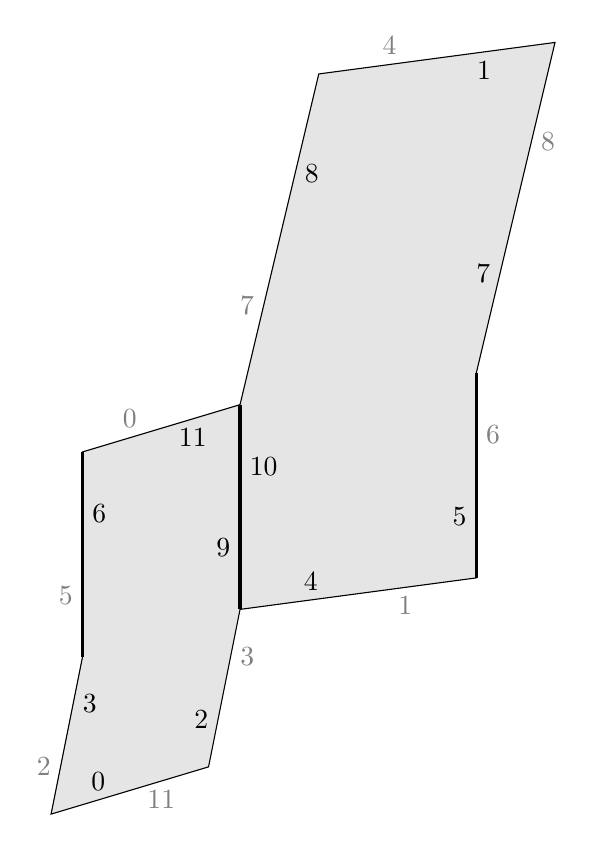
\begin{tikzpicture}[scale=2]
\coordinate (h0) at (1,.3);
\coordinate (mh0) at ($(0,0) - (h0)$);
\coordinate (h1) at (1.5,.2);
\coordinate (mh1) at ($(0,0) - (h1)$);
\coordinate (v0) at (0.2, 1);
\coordinate (mv0) at ($(0,0) - (v0)$);
\coordinate (v1) at (0,1.3);
\coordinate (mv1) at ($(0,0) - (v1)$);
\coordinate (v2) at (0.5,2.1);
\coordinate (mv2) at ($(0,0) - (v2)$);


\filldraw[draw=black,fill=gray!20]
(0,0) -- node[above,pos=0.3] {0} node[gray,below,pos=0.7] {11} ++(h0)
      -- node[left,pos=0.3] {2} node[gray,right,pos=0.7] {3} ++(v0)
      -- node[above,pos=0.3] {4} node[gray,below,pos=0.7] {1} ++(h1)
      -- node[left,pos=0.3] {5} node[gray,right,pos=0.7] {6} ++(v1)
      -- node[left,pos=0.3] {7} node[gray,right,pos=0.7] {8} ++(v2)
      -- node[below,pos=0.3] {1} node[gray,above,pos=0.7] {4} ++(mh1)
      -- node[right,pos=0.3] {8} node[gray,left,pos=0.7] {7} ++(mv2)
      -- node[below,pos=0.3] {11} node[gray,above,pos=0.7] {0} ++(mh0)
      -- node[right,pos=0.3] {6} node[gray,left,pos=0.7] {5} ++(mv1)
      -- node[right,pos=0.3] {3} node[gray,left,pos=0.7] {2} ++(mv0)
      -- cycle;

\draw ($(h0)+(v0)$) -- node[left,pos=0.3] {9} node[right,pos=0.7] {10} ++(v1);

\draw[very thick] (v0) -- ++(v1);
\draw[very thick] ($(h0)+(v0)$) -- ++(v1);
\draw[very thick] ($(h0)+(v0)+(h1)$) -- ++(v1);
\end{tikzpicture}\end{document}
